\documentclass[tikz,border=2pt]{standalone}
\usepackage{amsmath,amssymb}
\usepackage{tikz}
\usetikzlibrary{arrows.meta}

\begin{document}
% 1, 1.4, 1.41, 1.414, ... is Cauchy. In R it converges (to sqrt 2); in Q the would-be limit is a
% hole, so Q is not complete while R is.
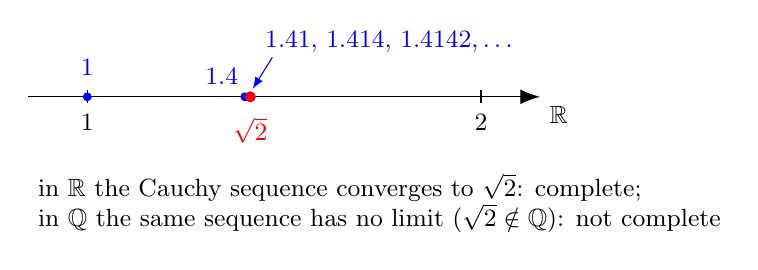
\begin{tikzpicture}[x=5cm, every node/.style={font=\small}]
	\draw[-{Latex[length=2.5mm]}] (0.85,0) -- (2.15,0) node[below right] {$\mathbb{R}$};
	\foreach \x/\l in {1/1, 2/2} {\draw (\x,0.08) -- (\x,-0.08); \node[below=3pt] at (\x,0) {\l};}
	\foreach \x in {1, 1.4, 1.41, 1.414, 1.4142} {\fill[blue] (\x,0) circle (1.6pt);}
	\node[blue, above=4pt] at (1,0) {$1$};
	\node[blue, anchor=south east, inner sep=1.5pt] at (1.395,0.1) {$1.4$};
	\node[blue, anchor=south west, inner sep=1.5pt] at (1.44,0.5) {$1.41,\,1.414,\,1.4142,\dots$};
	\draw[blue, -{Latex[length=1.5mm]}] (1.47,0.5) -- (1.42,0.1);
	\fill[red] (1.41421,0) circle (2pt);
	\node[red, below=4pt] at (1.41421,0) {$\sqrt2$};
	\node[anchor=north west, align=left] at (0.85,-0.85) {in $\mathbb{R}$ the Cauchy sequence converges to $\sqrt2$: complete;\\ in $\mathbb{Q}$ the same sequence has no limit ($\sqrt2\notin\mathbb{Q}$): not complete};
\end{tikzpicture}
\end{document}
